% Options for packages loaded elsewhere
% Options for packages loaded elsewhere
\PassOptionsToPackage{unicode}{hyperref}
\PassOptionsToPackage{hyphens}{url}
\PassOptionsToPackage{dvipsnames,svgnames,x11names}{xcolor}
%
\documentclass[
  letterpaper,
  DIV=11,
  numbers=noendperiod]{scrartcl}
\usepackage{xcolor}
\usepackage{amsmath,amssymb}
\setcounter{secnumdepth}{-\maxdimen} % remove section numbering
\usepackage{iftex}
\ifPDFTeX
  \usepackage[T1]{fontenc}
  \usepackage[utf8]{inputenc}
  \usepackage{textcomp} % provide euro and other symbols
\else % if luatex or xetex
  \usepackage{unicode-math} % this also loads fontspec
  \defaultfontfeatures{Scale=MatchLowercase}
  \defaultfontfeatures[\rmfamily]{Ligatures=TeX,Scale=1}
\fi
\usepackage{lmodern}
\ifPDFTeX\else
  % xetex/luatex font selection
\fi
% Use upquote if available, for straight quotes in verbatim environments
\IfFileExists{upquote.sty}{\usepackage{upquote}}{}
\IfFileExists{microtype.sty}{% use microtype if available
  \usepackage[]{microtype}
  \UseMicrotypeSet[protrusion]{basicmath} % disable protrusion for tt fonts
}{}
\makeatletter
\@ifundefined{KOMAClassName}{% if non-KOMA class
  \IfFileExists{parskip.sty}{%
    \usepackage{parskip}
  }{% else
    \setlength{\parindent}{0pt}
    \setlength{\parskip}{6pt plus 2pt minus 1pt}}
}{% if KOMA class
  \KOMAoptions{parskip=half}}
\makeatother
% Make \paragraph and \subparagraph free-standing
\makeatletter
\ifx\paragraph\undefined\else
  \let\oldparagraph\paragraph
  \renewcommand{\paragraph}{
    \@ifstar
      \xxxParagraphStar
      \xxxParagraphNoStar
  }
  \newcommand{\xxxParagraphStar}[1]{\oldparagraph*{#1}\mbox{}}
  \newcommand{\xxxParagraphNoStar}[1]{\oldparagraph{#1}\mbox{}}
\fi
\ifx\subparagraph\undefined\else
  \let\oldsubparagraph\subparagraph
  \renewcommand{\subparagraph}{
    \@ifstar
      \xxxSubParagraphStar
      \xxxSubParagraphNoStar
  }
  \newcommand{\xxxSubParagraphStar}[1]{\oldsubparagraph*{#1}\mbox{}}
  \newcommand{\xxxSubParagraphNoStar}[1]{\oldsubparagraph{#1}\mbox{}}
\fi
\makeatother

\usepackage{color}
\usepackage{fancyvrb}
\newcommand{\VerbBar}{|}
\newcommand{\VERB}{\Verb[commandchars=\\\{\}]}
\DefineVerbatimEnvironment{Highlighting}{Verbatim}{commandchars=\\\{\}}
% Add ',fontsize=\small' for more characters per line
\usepackage{framed}
\definecolor{shadecolor}{RGB}{241,243,245}
\newenvironment{Shaded}{\begin{snugshade}}{\end{snugshade}}
\newcommand{\AlertTok}[1]{\textcolor[rgb]{0.68,0.00,0.00}{#1}}
\newcommand{\AnnotationTok}[1]{\textcolor[rgb]{0.37,0.37,0.37}{#1}}
\newcommand{\AttributeTok}[1]{\textcolor[rgb]{0.40,0.45,0.13}{#1}}
\newcommand{\BaseNTok}[1]{\textcolor[rgb]{0.68,0.00,0.00}{#1}}
\newcommand{\BuiltInTok}[1]{\textcolor[rgb]{0.00,0.23,0.31}{#1}}
\newcommand{\CharTok}[1]{\textcolor[rgb]{0.13,0.47,0.30}{#1}}
\newcommand{\CommentTok}[1]{\textcolor[rgb]{0.37,0.37,0.37}{#1}}
\newcommand{\CommentVarTok}[1]{\textcolor[rgb]{0.37,0.37,0.37}{\textit{#1}}}
\newcommand{\ConstantTok}[1]{\textcolor[rgb]{0.56,0.35,0.01}{#1}}
\newcommand{\ControlFlowTok}[1]{\textcolor[rgb]{0.00,0.23,0.31}{\textbf{#1}}}
\newcommand{\DataTypeTok}[1]{\textcolor[rgb]{0.68,0.00,0.00}{#1}}
\newcommand{\DecValTok}[1]{\textcolor[rgb]{0.68,0.00,0.00}{#1}}
\newcommand{\DocumentationTok}[1]{\textcolor[rgb]{0.37,0.37,0.37}{\textit{#1}}}
\newcommand{\ErrorTok}[1]{\textcolor[rgb]{0.68,0.00,0.00}{#1}}
\newcommand{\ExtensionTok}[1]{\textcolor[rgb]{0.00,0.23,0.31}{#1}}
\newcommand{\FloatTok}[1]{\textcolor[rgb]{0.68,0.00,0.00}{#1}}
\newcommand{\FunctionTok}[1]{\textcolor[rgb]{0.28,0.35,0.67}{#1}}
\newcommand{\ImportTok}[1]{\textcolor[rgb]{0.00,0.46,0.62}{#1}}
\newcommand{\InformationTok}[1]{\textcolor[rgb]{0.37,0.37,0.37}{#1}}
\newcommand{\KeywordTok}[1]{\textcolor[rgb]{0.00,0.23,0.31}{\textbf{#1}}}
\newcommand{\NormalTok}[1]{\textcolor[rgb]{0.00,0.23,0.31}{#1}}
\newcommand{\OperatorTok}[1]{\textcolor[rgb]{0.37,0.37,0.37}{#1}}
\newcommand{\OtherTok}[1]{\textcolor[rgb]{0.00,0.23,0.31}{#1}}
\newcommand{\PreprocessorTok}[1]{\textcolor[rgb]{0.68,0.00,0.00}{#1}}
\newcommand{\RegionMarkerTok}[1]{\textcolor[rgb]{0.00,0.23,0.31}{#1}}
\newcommand{\SpecialCharTok}[1]{\textcolor[rgb]{0.37,0.37,0.37}{#1}}
\newcommand{\SpecialStringTok}[1]{\textcolor[rgb]{0.13,0.47,0.30}{#1}}
\newcommand{\StringTok}[1]{\textcolor[rgb]{0.13,0.47,0.30}{#1}}
\newcommand{\VariableTok}[1]{\textcolor[rgb]{0.07,0.07,0.07}{#1}}
\newcommand{\VerbatimStringTok}[1]{\textcolor[rgb]{0.13,0.47,0.30}{#1}}
\newcommand{\WarningTok}[1]{\textcolor[rgb]{0.37,0.37,0.37}{\textit{#1}}}

\usepackage{longtable,booktabs,array}
\usepackage{calc} % for calculating minipage widths
% Correct order of tables after \paragraph or \subparagraph
\usepackage{etoolbox}
\makeatletter
\patchcmd\longtable{\par}{\if@noskipsec\mbox{}\fi\par}{}{}
\makeatother
% Allow footnotes in longtable head/foot
\IfFileExists{footnotehyper.sty}{\usepackage{footnotehyper}}{\usepackage{footnote}}
\makesavenoteenv{longtable}
\usepackage{graphicx}
\makeatletter
\newsavebox\pandoc@box
\newcommand*\pandocbounded[1]{% scales image to fit in text height/width
  \sbox\pandoc@box{#1}%
  \Gscale@div\@tempa{\textheight}{\dimexpr\ht\pandoc@box+\dp\pandoc@box\relax}%
  \Gscale@div\@tempb{\linewidth}{\wd\pandoc@box}%
  \ifdim\@tempb\p@<\@tempa\p@\let\@tempa\@tempb\fi% select the smaller of both
  \ifdim\@tempa\p@<\p@\scalebox{\@tempa}{\usebox\pandoc@box}%
  \else\usebox{\pandoc@box}%
  \fi%
}
% Set default figure placement to htbp
\def\fps@figure{htbp}
\makeatother





\setlength{\emergencystretch}{3em} % prevent overfull lines

\providecommand{\tightlist}{%
  \setlength{\itemsep}{0pt}\setlength{\parskip}{0pt}}



 


\KOMAoption{captions}{tableheading}
\makeatletter
\@ifpackageloaded{tcolorbox}{}{\usepackage[skins,breakable]{tcolorbox}}
\@ifpackageloaded{fontawesome5}{}{\usepackage{fontawesome5}}
\definecolor{quarto-callout-color}{HTML}{909090}
\definecolor{quarto-callout-note-color}{HTML}{0758E5}
\definecolor{quarto-callout-important-color}{HTML}{CC1914}
\definecolor{quarto-callout-warning-color}{HTML}{EB9113}
\definecolor{quarto-callout-tip-color}{HTML}{00A047}
\definecolor{quarto-callout-caution-color}{HTML}{FC5300}
\definecolor{quarto-callout-color-frame}{HTML}{acacac}
\definecolor{quarto-callout-note-color-frame}{HTML}{4582ec}
\definecolor{quarto-callout-important-color-frame}{HTML}{d9534f}
\definecolor{quarto-callout-warning-color-frame}{HTML}{f0ad4e}
\definecolor{quarto-callout-tip-color-frame}{HTML}{02b875}
\definecolor{quarto-callout-caution-color-frame}{HTML}{fd7e14}
\makeatother
\makeatletter
\@ifpackageloaded{caption}{}{\usepackage{caption}}
\AtBeginDocument{%
\ifdefined\contentsname
  \renewcommand*\contentsname{Table of contents}
\else
  \newcommand\contentsname{Table of contents}
\fi
\ifdefined\listfigurename
  \renewcommand*\listfigurename{List of Figures}
\else
  \newcommand\listfigurename{List of Figures}
\fi
\ifdefined\listtablename
  \renewcommand*\listtablename{List of Tables}
\else
  \newcommand\listtablename{List of Tables}
\fi
\ifdefined\figurename
  \renewcommand*\figurename{Figure}
\else
  \newcommand\figurename{Figure}
\fi
\ifdefined\tablename
  \renewcommand*\tablename{Table}
\else
  \newcommand\tablename{Table}
\fi
}
\@ifpackageloaded{float}{}{\usepackage{float}}
\floatstyle{ruled}
\@ifundefined{c@chapter}{\newfloat{codelisting}{h}{lop}}{\newfloat{codelisting}{h}{lop}[chapter]}
\floatname{codelisting}{Listing}
\newcommand*\listoflistings{\listof{codelisting}{List of Listings}}
\makeatother
\makeatletter
\makeatother
\makeatletter
\@ifpackageloaded{caption}{}{\usepackage{caption}}
\@ifpackageloaded{subcaption}{}{\usepackage{subcaption}}
\makeatother
\usepackage{bookmark}
\IfFileExists{xurl.sty}{\usepackage{xurl}}{} % add URL line breaks if available
\urlstyle{same}
\hypersetup{
  pdftitle={PREACT-digital: Feature Database Documentation},
  pdfauthor={Leona Hammelrath; Tessa Meyer},
  colorlinks=true,
  linkcolor={blue},
  filecolor={Maroon},
  citecolor={Blue},
  urlcolor={Blue},
  pdfcreator={LaTeX via pandoc}}


\title{PREACT-digital: Feature Database Documentation}
\author{Leona Hammelrath \and Tessa Meyer}
\date{2025-03-03}
\begin{document}
\maketitle


\subsection{Introduction}\label{introduction}

Welcome to the documentation for the PREACT-digital study
(\href{https://doi.org/10.1101/2025.03.14.25323957}{study protocol}).

\subsection{Design}\label{design}

\subsubsection{Longitudinal study design
(PREACT-digital)}\label{longitudinal-study-design-preact-digital}

\begin{figure}[H]

{\centering 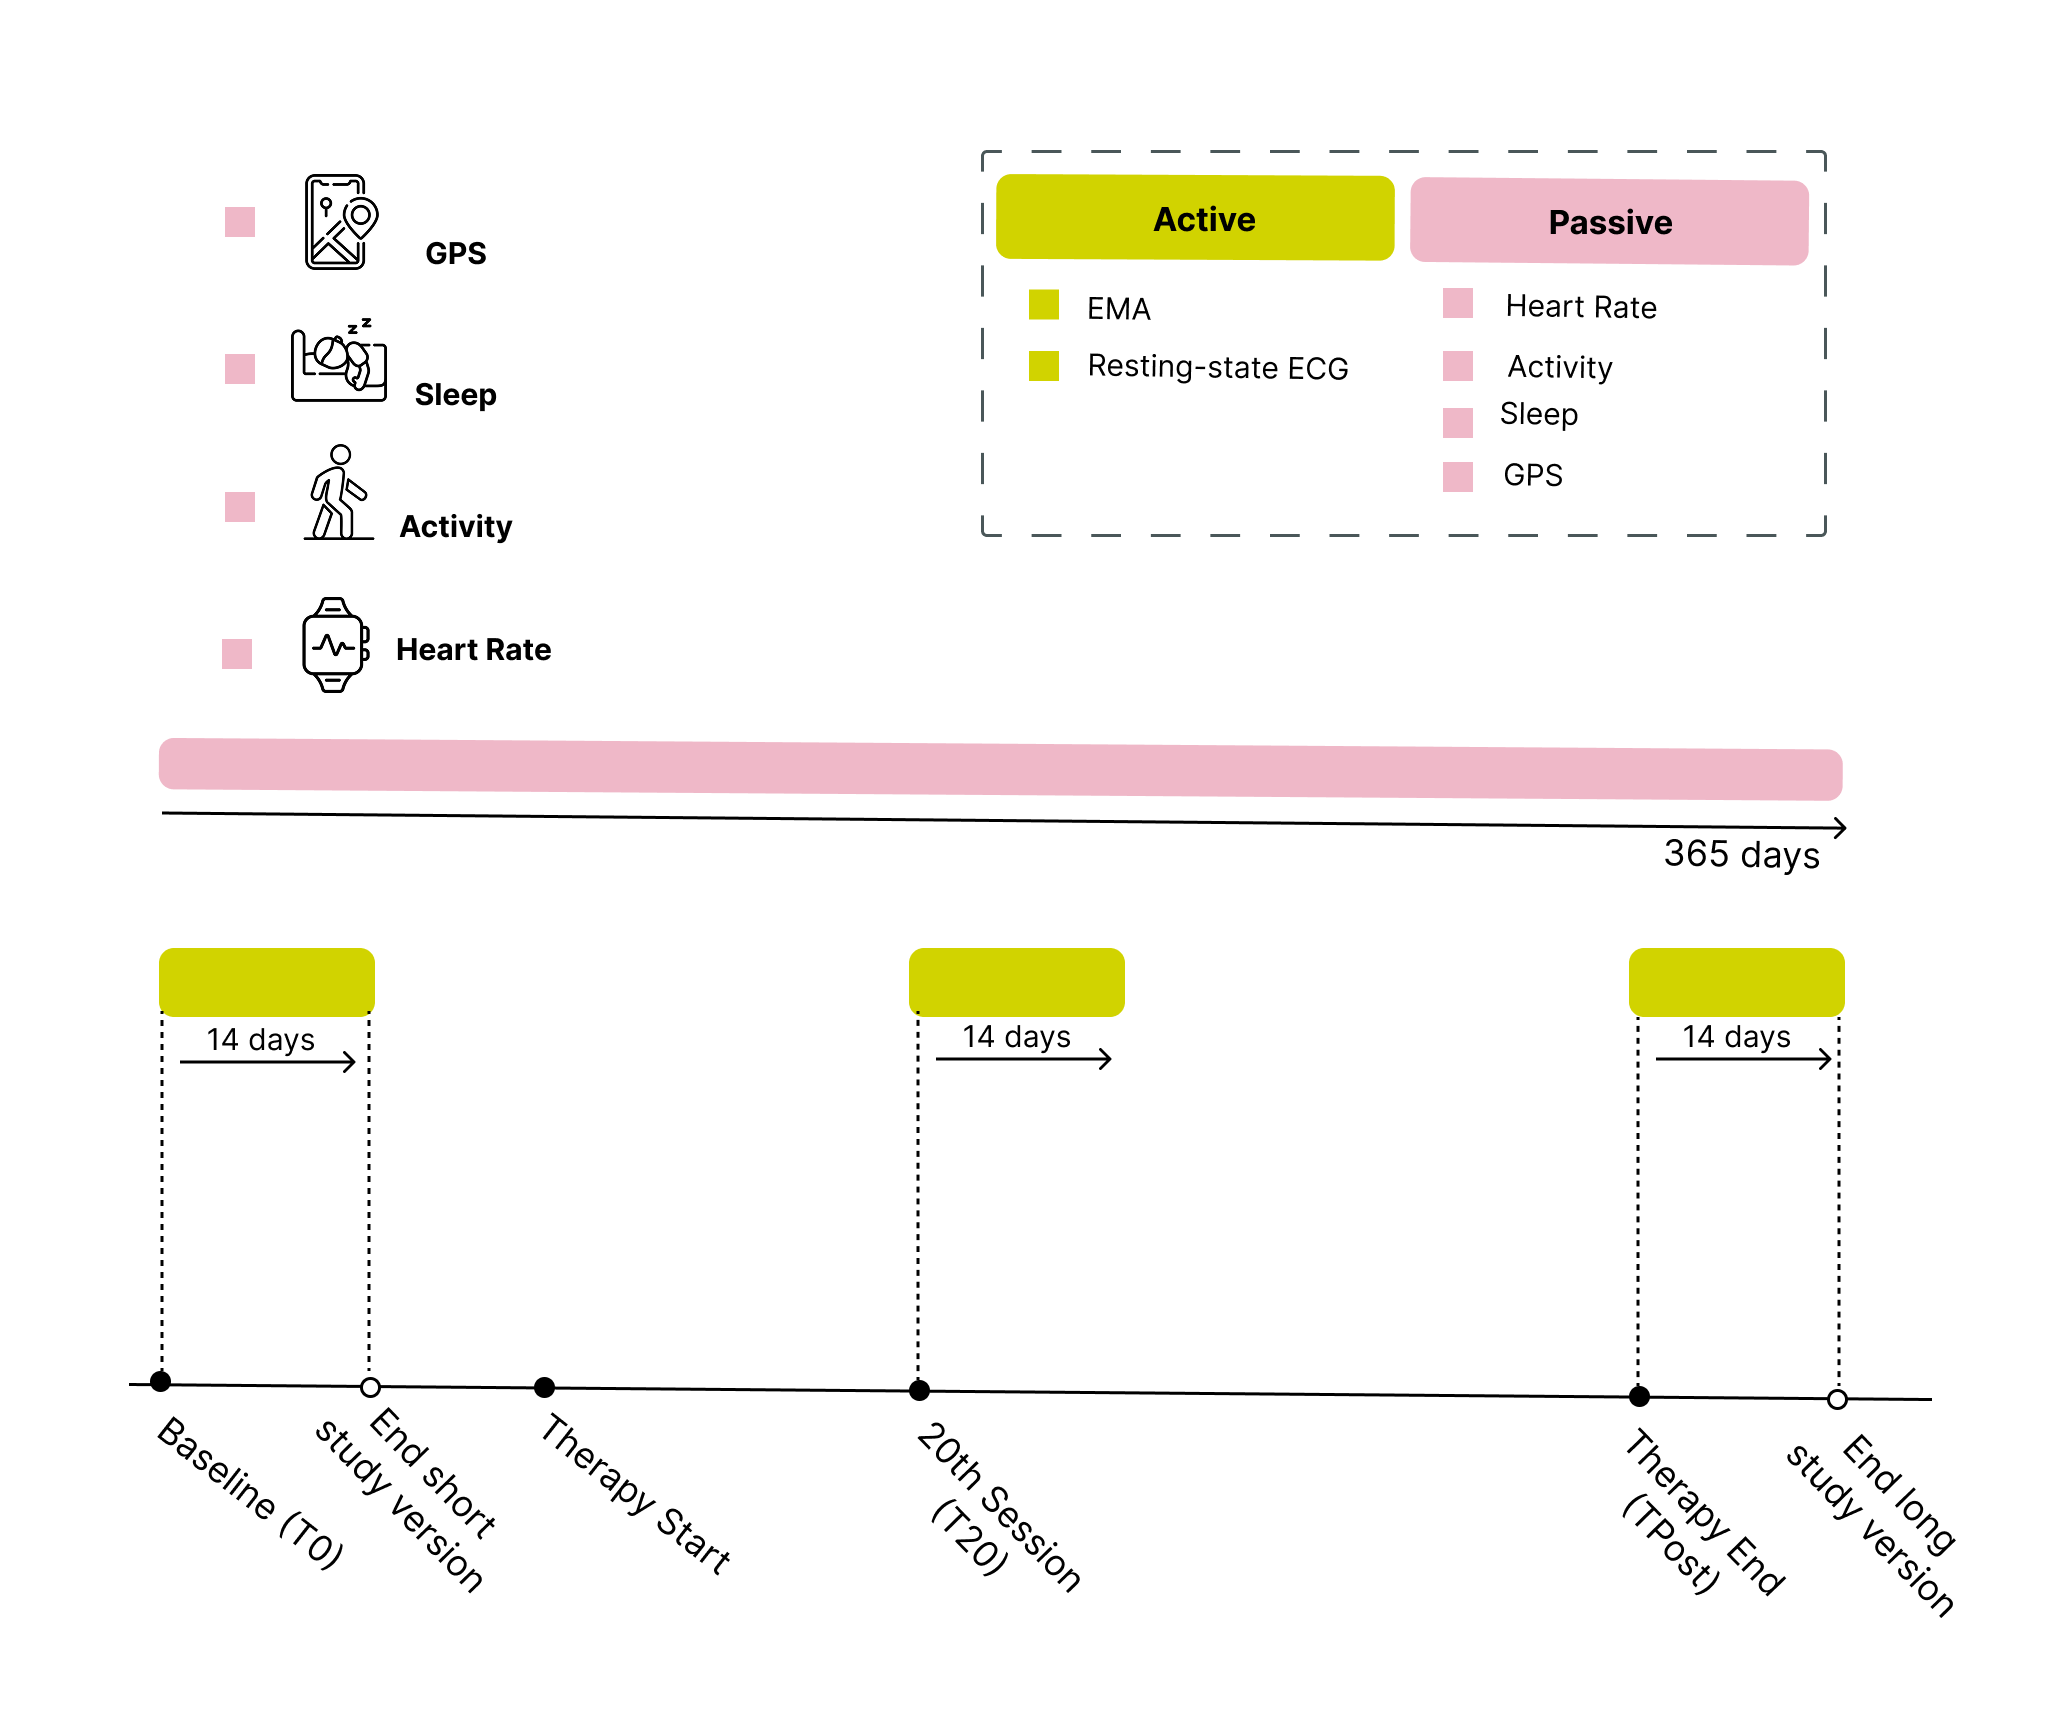
\includegraphics[width=6.25in,height=\textheight,keepaspectratio]{images/preact-digital_study-procedure_small.png}

}

\caption{Caption describing the figure}

\end{figure}%

\begin{center}\rule{0.5\linewidth}{0.5pt}\end{center}

\begin{tcolorbox}[enhanced jigsaw, titlerule=0mm, colframe=quarto-callout-tip-color-frame, bottomtitle=1mm, left=2mm, arc=.35mm, toptitle=1mm, breakable, opacityback=0, opacitybacktitle=0.6, title=\textcolor{quarto-callout-tip-color}{\faLightbulb}\hspace{0.5em}{Glossary}, rightrule=.15mm, colback=white, leftrule=.75mm, toprule=.15mm, colbacktitle=quarto-callout-tip-color!10!white, bottomrule=.15mm, coltitle=black]

\begin{itemize}
\item
  \textbf{beep} =
\item
  \textbf{measurement burst} =
\item
  \ldots{}
\end{itemize}

\end{tcolorbox}

\subsection{Data Structure}\label{data-structure}

\textbf{Folder Structure on High Performance Cluster (HPC)} {[}wip{]}

\begin{Shaded}
\begin{Highlighting}[]
\NormalTok{SP6}\OperatorTok{/}
    \OperatorTok{|{-}}\NormalTok{ processed}\OperatorTok{/}
        \OperatorTok{|{-}}\NormalTok{ passive}\OperatorTok{/}
            \OperatorTok{|{-}}\NormalTok{ epoch                        }\CommentTok{\# not aggregated; most finegrained resolution}
                \OperatorTok{|{-}}\NormalTok{ activity\_epoch}
                \OperatorTok{|{-}}\NormalTok{ heart\_rate\_epoch}
                \OperatorTok{|{-}}\NormalTok{ ecg\_epoch}
                \OperatorTok{|{-}}\NormalTok{ gps\_epoch}
            \OperatorTok{|{-}}\NormalTok{ daily                        }\CommentTok{\# daily aggregates}
                \OperatorTok{|{-}}\NormalTok{ activity\_daily}
                \OperatorTok{|{-}}\NormalTok{ heart\_rate\_daily}
                \OperatorTok{|{-}}\NormalTok{ ecg\_daily}
                \OperatorTok{|{-}}\NormalTok{ gps\_daily}
        \OperatorTok{|{-}}\NormalTok{ ema}
                \OperatorTok{|{-}}\NormalTok{ ema\_beep                 }\CommentTok{\# not aggregated; most finegrained resolution   }
                \OperatorTok{|{-}}\NormalTok{ ema\_daily                }\CommentTok{\# daily aggregate}
                \OperatorTok{|{-}}\NormalTok{ ema\_burst                }\CommentTok{\# burst aggregate}
                \OperatorTok{|{-}}\NormalTok{ ema\_meta                 }\CommentTok{\# technical meta data}
        \OperatorTok{|{-}}\NormalTok{ ecg}
                \OperatorTok{|{-}}\NormalTok{ ecg\_raw                  }\CommentTok{\# raw data (sampling rate: 300 Hz; 9000 data points/30sec)}
                \OperatorTok{|{-}}\NormalTok{ ecg\_processed            }\CommentTok{\# processed, e.g. heart rate variability (hrv) }
        \OperatorTok{|{-}}\NormalTok{ meta}
                \OperatorTok{|{-}}\NormalTok{ monitoring               }\CommentTok{\# study monitoring}
\end{Highlighting}
\end{Shaded}

\subsection{EMA Data}\label{ema-data}

This section outlines the EMA data sets (\hyperref[files]{files}) in
detail and provides a thorough description of the eight
\hyperref[emaconstructs]{EMA constructs} and a
\hyperref[emaconstructs]{item-level overview}.

\subsubsection{Data sets}\label{data-sets}

\subparagraph{Files:}\label{files}

\begin{itemize}
\tightlist
\item
  \texttt{ema\_beep.pkl}
\item
  \texttt{ema\_meta.pkl}
\end{itemize}

\textbf{Details} \texttt{ema\_content.pkl} \textbf{file:}

Show details

\begin{longtable}[]{@{}
  >{\raggedright\arraybackslash}p{(\linewidth - 10\tabcolsep) * \real{0.0806}}
  >{\raggedright\arraybackslash}p{(\linewidth - 10\tabcolsep) * \real{0.2097}}
  >{\raggedright\arraybackslash}p{(\linewidth - 10\tabcolsep) * \real{0.2097}}
  >{\raggedright\arraybackslash}p{(\linewidth - 10\tabcolsep) * \real{0.1774}}
  >{\raggedright\arraybackslash}p{(\linewidth - 10\tabcolsep) * \real{0.1774}}
  >{\raggedright\arraybackslash}p{(\linewidth - 10\tabcolsep) * \real{0.1452}}@{}}
\toprule\noalign{}
\begin{minipage}[b]{\linewidth}\raggedright
No.
\end{minipage} & \begin{minipage}[b]{\linewidth}\raggedright
Column name
\end{minipage} & \begin{minipage}[b]{\linewidth}\raggedright
Description
\end{minipage} & \begin{minipage}[b]{\linewidth}\raggedright
Data type
\end{minipage} & \begin{minipage}[b]{\linewidth}\raggedright
Scale level
\end{minipage} & \begin{minipage}[b]{\linewidth}\raggedright
Variable Level
\end{minipage} \\
\midrule\noalign{}
\endhead
\bottomrule\noalign{}
\endlastfoot
1 & \texttt{id} & Unique identifier wearable and ema data within
subproject 6 (SP6) & \texttt{str} & & \\
2 & \texttt{for\_id} & Unique identifier across all PREACT subprojects
and redcap & \texttt{str} & & \\
3 & \texttt{timestamp\_item\_completion} & Timestamp at which a single
item was completed & \texttt{datetime64} & interval & \\
4 & \texttt{timestamp\_beep\_completion} & Timestamp at which a beep was
completed & \texttt{datetime64} & interval & \\
5 & \texttt{timestamp\_beep\_expiration} & Timestamp at which the
processing of the beep has expired (a beep expires after 30 min) &
\texttt{datetime64} & interval & \\
6 & \texttt{measurment\_burst} & Measurement burst describes the
measurement point in the longitudinal study {[}Baseline (T0), after 20
therapy sessions (T20), or after therapy end respectively 365 days after
therapy start (TPost){]} & \texttt{int} & ordinal & 0 = T0 1 = T20 2 =
TPost \\
7 & \texttt{schedule\_chronotype} & Depending on their individual
sleep-wake rhythm participants can choose to receive beeps between 07:30
and 21:30 (lark) or 09:30 and 22:30 (owl) & \texttt{int} & nominal & 24
= T0 lark 25 = T0 owl 33 = T20 lark 34 = T20 owl 38 = TPost lark 39 =
TPost owl \\
8 & \texttt{response} & Chosen response by participant & \texttt{int} &
ordinal, nominal, binary & \\
9 & \texttt{item} & Question/item title & \texttt{str} & & \\
10 & \texttt{beep\_per\_person\_id} & Unique beep identifier. Date and
number of beep per ID & \texttt{str} & & \\
11 & \texttt{date} & Date on which the question/item was generated &
\texttt{datetime64} & interval & \\
12 & \texttt{study\_version} & Study version (short version: includes
Baseline (T0), long version: includes Baseline (T0), T20 and TPost) &
\texttt{int} & nominal & 1= long 2 = short \\
13 & \texttt{ema\_burst\_start} & Absolute start EMA measurement burst
(i.e.~defined start according to study protocol) & \texttt{datetime64} &
interval & \\
14 & \texttt{ema\_burst\_end} & Absolute end EMA measurement burst
(i.e.~defined end according to study protocol) & \texttt{datetime64} &
interval & \\
15 & \texttt{season} & Describes the four seasons & \texttt{int} &
nominal & 1 = Spring 2 = Summer 3 = Fall 4 = Winter \\
16 & \texttt{time\_of\_day} & Time of day stratified into five
categories (Early Morning = 00:00 - 00:00, Morning = 00:00 - 00:00,
Afternoon = 00:00 - 00:00, Evening = 00:00 - 00:00, Night = 00:00 -
00:00) & \texttt{int} & nominal & 1 = Early Morning 2 = Morning 3 =
Afternoon 4 = Evening 5 = Night \\
17 & \texttt{weekend} & Does the timestamp in the time series describes
a day at the weekend? & \texttt{int} & nominal & 0 = No 1 = Yes \\
18 & \texttt{nr\_beep\_daily} & Number of questionnaire/beep within a
day & \texttt{int} & ordinal & 1 - 8 \\
19 & \texttt{n\_beeps\_completed} & Number of questionnaires/beeps
completed by a person within a day & \texttt{int} & ordinal & 1 - 9 \\
20 & \texttt{ema\_relat\_burst\_start} & Relative start EMA measurement
burst (i.e.~actual start) & \texttt{datetime64} & interval & \\
21 & \texttt{ema\_relat\_burst\_end} & Relative end EMA measurement
burst (i.e.~actual end) & \texttt{datetime64} & interval & \\
22 & \texttt{absolute\_day\_index} & Day since expected (absolute) start
& \texttt{int} & ratio & 1 - 16 \\
23 & \texttt{relative\_day\_index} & Day since actual (relative) start &
\texttt{int} & ratio & 1 - 16 \\
\end{longtable}

\textbf{Details} \texttt{ema\_meta.pkl} \textbf{file:}

Show details

\begin{longtable}[]{@{}
  >{\raggedright\arraybackslash}p{(\linewidth - 10\tabcolsep) * \real{0.0806}}
  >{\raggedright\arraybackslash}p{(\linewidth - 10\tabcolsep) * \real{0.2097}}
  >{\raggedright\arraybackslash}p{(\linewidth - 10\tabcolsep) * \real{0.2097}}
  >{\raggedright\arraybackslash}p{(\linewidth - 10\tabcolsep) * \real{0.1774}}
  >{\raggedright\arraybackslash}p{(\linewidth - 10\tabcolsep) * \real{0.1774}}
  >{\raggedright\arraybackslash}p{(\linewidth - 10\tabcolsep) * \real{0.1452}}@{}}
\toprule\noalign{}
\begin{minipage}[b]{\linewidth}\raggedright
No.
\end{minipage} & \begin{minipage}[b]{\linewidth}\raggedright
Column name
\end{minipage} & \begin{minipage}[b]{\linewidth}\raggedright
Description
\end{minipage} & \begin{minipage}[b]{\linewidth}\raggedright
Data type
\end{minipage} & \begin{minipage}[b]{\linewidth}\raggedright
Scale level
\end{minipage} & \begin{minipage}[b]{\linewidth}\raggedright
Variable Level
\end{minipage} \\
\midrule\noalign{}
\endhead
\bottomrule\noalign{}
\endlastfoot
1 & \texttt{id} & Unique identifier wearable and ema data within
subproject 6 (SP6) & \texttt{str} & & \\
2 & \texttt{for\_id} & Unique identifier across all PREACT subprojects
and redcap & \texttt{str} & & \\
3 & \texttt{response\_text} & Response displayed on device &
\texttt{str} & & \\
4 & \texttt{item\_code\_map} & Numerical item code mapping &
\texttt{int} & {[}insert{]} & nominal \\
5 & \texttt{beep\_type} & & \texttt{int} & & nominal \\
6 & \texttt{beep\_type\_name} & Name of the questionnaire & \texttt{str}
& & \\
7 & \texttt{item\_order} & Order in which the items are displayed &
\texttt{int} & 0 - 8 & \\
8 & \texttt{beep\_num\_run} & How many times a beep was opend before
completion. Unique per answer. One beep can have multiple runs until
completion & \texttt{int} & & \\
\end{longtable}

\subsubsection{Methods: Hierarchical Data
Structure}\label{methods-hierarchical-data-structure}

\begin{enumerate}
\def\labelenumi{\arabic{enumi}.}
\tightlist
\item
  \textbf{Level 1: Measurements (Observations)}

  \begin{itemize}
  \tightlist
  \item
    Each person records data 8x/day over 14 days
  \item
    This results in 112 measurements per wave (8x14)
  \end{itemize}
\item
  \textbf{Level 2: Days}

  \begin{itemize}
  \tightlist
  \item
    Measurements (Level 1) are nested within days (Level 2)
  \item
    Each wave has 14 days
  \end{itemize}
\item
  \textbf{Level 3: Waves (Measurement points)}

  \begin{itemize}
  \tightlist
  \item
    Each person goes thorugh three waves (long version)
  \item
    Days (Level 2) are nested within waves (Level 3)
  \end{itemize}
\item
  \textbf{Level 4: Individuals (Participants)}

  \begin{itemize}
  \tightlist
  \item
    Waves (Level 3) are nested within participants (Level 4)
  \end{itemize}
\end{enumerate}

\begin{center}\rule{0.5\linewidth}{0.5pt}\end{center}

\subsubsection{EMA constructs and item-level
overview}\label{emaconstructs}

The EMA measurement includes the following constructs:

\begin{enumerate}
\def\labelenumi{\arabic{enumi}.}
\tightlist
\item
  \hyperref[affect]{Affect}
\item
  \hyperref[emotion-regulation]{Emotion regulation}
\item
  \hyperref[situational-context]{Situational context}
\item
  \hyperref[significant-events]{Significant events}
\item
  \hyperref[social-context]{Social context}
\item
  \hyperref[therapeutic-agency]{Therapeutic agency}
\item
  \hyperref[physical-fitness]{Physical fitness}
\item
  \hyperref[ecg-control]{ECG control}
\end{enumerate}

\paragraph{Affect}\label{affect}

\begin{itemize}
\item
  Description: At each beep, participants were asked about their current
  affective state
\item
  Construct: PANAS-X subscales
  \href{https://doi.org/10.1037/pas0001231}{Haney et al.~(2023)}
\item
  17 Items
\end{itemize}

Show Items

\begin{longtable}[]{@{}
  >{\raggedright\arraybackslash}p{(\linewidth - 8\tabcolsep) * \real{0.1475}}
  >{\raggedright\arraybackslash}p{(\linewidth - 8\tabcolsep) * \real{0.1148}}
  >{\raggedright\arraybackslash}p{(\linewidth - 8\tabcolsep) * \real{0.1311}}
  >{\raggedright\arraybackslash}p{(\linewidth - 8\tabcolsep) * \real{0.2951}}
  >{\raggedright\arraybackslash}p{(\linewidth - 8\tabcolsep) * \real{0.3115}}@{}}
\toprule\noalign{}
\begin{minipage}[b]{\linewidth}\raggedright
Variable
\end{minipage} & \begin{minipage}[b]{\linewidth}\raggedright
Item
\end{minipage} & \begin{minipage}[b]{\linewidth}\raggedright
Scale
\end{minipage} & \begin{minipage}[b]{\linewidth}\raggedright
Scale Endpoints
\end{minipage} & \begin{minipage}[b]{\linewidth}\raggedright
Measurement Time
\end{minipage} \\
\midrule\noalign{}
\endhead
\bottomrule\noalign{}
\endlastfoot
& How \ldots{} do you feel right now? & & & \\
\texttt{anxious} & anxious & 1-2-3-4-5-6-7 & not at all - very much &
all beeps \\
\texttt{nervous} & nervous & 1-2-3-4-5-6-7 & not at all - very much &
all beeps \\
\texttt{attentive} & attentive & 1-2-3-4-5-6-7 & not at all - very much
& all beeps \\
\texttt{relaxed} & relaxed & 1-2-3-4-5-6-7 & not at all - very much &
all beeps \\
\texttt{calm} & calm & 1-2-3-4-5-6-7 & not at all - very much & all
beeps \\
\texttt{irritable} & irritable & 1-2-3-4-5-6-7 & not at all - very much
& all beeps \\
\texttt{angry} & angry & 1-2-3-4-5-6-7 & not at all - very much & all
beeps \\
\texttt{fatigue} & fatigue & 1-2-3-4-5-6-7 & not at all - very much &
all beeps \\
\texttt{cheerful} & cheerful & 1-2-3-4-5-6-7 & not at all - very much &
all beeps \\
\texttt{happy} & happy & 1-2-3-4-5-6-7 & not at all - very much & all
beeps \\
\texttt{ashamed} & ashamed & 1-2-3-4-5-6-7 & not at all - very much &
all beeps \\
\texttt{dissatisfied\_myself} & dissatisfied with myself & 1-2-3-4-5-6-7
& not at all - very much & all beeps \\
\texttt{self\_confident} & self-confident & 1-2-3-4-5-6-7 & not at all -
very much & all beeps \\
\texttt{shy} & shy & 1-2-3-4-5-6-7 & not at all - very much & all
beeps \\
\texttt{downcast} & downcast & 1-2-3-4-5-6-7 & not at all - very much &
all beeps \\
\texttt{sad} & sad & 1-2-3-4-5-6-7 & not at all - very much & all
beeps \\
\texttt{lonely} & lonely & 1-2-3-4-5-6-7 & not at all - very much & all
beeps \\
\end{longtable}

\paragraph{Emotion regulation}\label{emotion-regulation}

\begin{itemize}
\item
  Description: At each beep, participants were asked to rate the
  intensity and controllability of their most negative thought since the
  last beep. Then, we assessed the use of different ER strategies since
  the last beep
\item
  Construct: RESS-EMA scale
  \href{https://doi.org/10.1027/1015-5759/a000595}{Medland et
  al.~(2020)}
\item
  6 Items (covering reappraisal, rumination, suppression, distraction,
  relaxation, acceptance)
\end{itemize}

Show Items

\begin{longtable}[]{@{}
  >{\raggedright\arraybackslash}p{(\linewidth - 8\tabcolsep) * \real{0.1475}}
  >{\raggedright\arraybackslash}p{(\linewidth - 8\tabcolsep) * \real{0.1148}}
  >{\raggedright\arraybackslash}p{(\linewidth - 8\tabcolsep) * \real{0.1311}}
  >{\raggedright\arraybackslash}p{(\linewidth - 8\tabcolsep) * \real{0.2951}}
  >{\raggedright\arraybackslash}p{(\linewidth - 8\tabcolsep) * \real{0.3115}}@{}}
\toprule\noalign{}
\begin{minipage}[b]{\linewidth}\raggedright
Variable
\end{minipage} & \begin{minipage}[b]{\linewidth}\raggedright
Item
\end{minipage} & \begin{minipage}[b]{\linewidth}\raggedright
Scale
\end{minipage} & \begin{minipage}[b]{\linewidth}\raggedright
Scale Endpoints
\end{minipage} & \begin{minipage}[b]{\linewidth}\raggedright
Measurement Time
\end{minipage} \\
\midrule\noalign{}
\endhead
\bottomrule\noalign{}
\endlastfoot
& Think about the strongest negative feeling since the last beep
{[}since waking up{]}. & & & \\
\texttt{er\_intensity} & How intense was this feeling? & 1-2-3-4-5-6-7
(1 = neutral) & not at all - very much & all beeps (except the first of
the day) \\
\texttt{er\_intensity\_morning} & How intense was this feeling? &
1-2-3-4-5-6-7 (1 = neutral) & not at all - very much & first beep of the
day \\
\texttt{er\_control} & How controllable was the situation that triggered
this feeling? & 1-2-3-4-5-6-7 (4 = neutral) & not at all - very much &
all beeps (except the first of the day) \\
\texttt{er\_control\_morning} & How controllable was the situation that
triggered this feeling? & 1-2-3-4-5-6-7 (4 = neutral) & not at all -
very much & first beep of the day \\
& As a reaction to the negative feeling \ldots{} & & & \\
\texttt{er\_relaxation} & I tried to breathe deeply & 1-2-3-4-5-6-7 &
not at all - very much & all beeps \\
\texttt{er\_rumination} & I kept thinking about what was bothering me &
1-2-3-4-5-6-7 & not at all - very much & all beeps \\
\texttt{er\_reappraisal} & I considered the situation from different
perspectives & 1-2-3-4-5-6-7 & not at all - very much & all beeps \\
\texttt{er\_distraction} & I tried to distract myself & 1-2-3-4-5-6-7 &
not at all - very much & all beeps \\
\texttt{er\_suppression} & I tried to hide my feelings & 1-2-3-4-5-6-7 &
not at all - very much & all beeps \\
\texttt{er\_acceptance} & I tried to accept the situation &
1-2-3-4-5-6-7 & not at all - very much & all beeps \\
\end{longtable}

\paragraph{Situational Context}\label{situational-context}

\begin{itemize}
\item
  Description: At each beep, participants were asked to specify
  activities they had pursued in the preceding 2 hours from a given set
  of 9 common activities. Participants were able to select multiple
  options simultaneously. Subsequently, they were asked to evaluate how
  much they enjoyed the respective activities
\item
  Construct: Self-constructed, based on the DIAMONDS scale
  \href{https://doi.org/10.1027/1015-5759/a000245}{Rauthmann \& Sherman
  (2016)} and the WARN-D study protocol
  \href{https://osf.io/preprints/psyarxiv/9qcvs_v1}{Fried et
  al.~(2022)}, a similar longitudinal digital phenotyping study. We
  aimed to find a balance between sparsity of items and high degree of
  situational coverage.
\item
  2 Items
\end{itemize}

Show Items

\begin{longtable}[]{@{}
  >{\raggedright\arraybackslash}p{(\linewidth - 8\tabcolsep) * \real{0.1475}}
  >{\raggedright\arraybackslash}p{(\linewidth - 8\tabcolsep) * \real{0.1148}}
  >{\raggedright\arraybackslash}p{(\linewidth - 8\tabcolsep) * \real{0.1475}}
  >{\raggedright\arraybackslash}p{(\linewidth - 8\tabcolsep) * \real{0.2787}}
  >{\raggedright\arraybackslash}p{(\linewidth - 8\tabcolsep) * \real{0.3115}}@{}}
\toprule\noalign{}
\begin{minipage}[b]{\linewidth}\raggedright
Variable
\end{minipage} & \begin{minipage}[b]{\linewidth}\raggedright
Item
\end{minipage} & \begin{minipage}[b]{\linewidth}\raggedright
Scale
\end{minipage} & \begin{minipage}[b]{\linewidth}\raggedright
Scale Endpoints
\end{minipage} & \begin{minipage}[b]{\linewidth}\raggedright
Measurement Time
\end{minipage} \\
\midrule\noalign{}
\endhead
\bottomrule\noalign{}
\endlastfoot
& How did you spent the time since the last beep {[}since waking up{]}?
(Multiple answers possible) & & & \\
\texttt{situation\_1} & {[} {]} Work or study {[} {]} Housework or
errands {[} {]} Caring for children/relatives {[} {]}
Eating/drinking/personal hygiene {[} {]} On the move (e.g., in the
subway) {[} {]} Smartphone/social media {[} {]} Leisure activity, rather
passive (e.g., watching a movie, reading) {[} {]} Leisure activity,
rather active (e.g., sports, outings) {[} {]} Something else & & & all
beeps (except the first of the day) \\
\texttt{situation\_1\_morning} & cf.~above & & & first beep of the
day \\
\texttt{situation\_2} & How much did you enjoy this activity? & -2, -1,
0, 1, 2 & not at all - very much & all beeps (except the first of the
day) \\
\texttt{situation\_2\_morning} & cf.~above & -2, -1, 0, 1, 2 & not at
all - very much & first beep of the day \\
\end{longtable}

\paragraph{Significant Events}\label{significant-events}

\begin{itemize}
\item
  Description: Participants were asked to think about the most important
  event since the last beep and how pleasant they perceived it
\item
  Construct: Self-constructed
\item
  1 Items
\end{itemize}

Show Items

\begin{longtable}[]{@{}
  >{\raggedright\arraybackslash}p{(\linewidth - 8\tabcolsep) * \real{0.1475}}
  >{\raggedright\arraybackslash}p{(\linewidth - 8\tabcolsep) * \real{0.1148}}
  >{\raggedright\arraybackslash}p{(\linewidth - 8\tabcolsep) * \real{0.1475}}
  >{\raggedright\arraybackslash}p{(\linewidth - 8\tabcolsep) * \real{0.2787}}
  >{\raggedright\arraybackslash}p{(\linewidth - 8\tabcolsep) * \real{0.3115}}@{}}
\toprule\noalign{}
\begin{minipage}[b]{\linewidth}\raggedright
Variable
\end{minipage} & \begin{minipage}[b]{\linewidth}\raggedright
Item
\end{minipage} & \begin{minipage}[b]{\linewidth}\raggedright
Scale
\end{minipage} & \begin{minipage}[b]{\linewidth}\raggedright
Scale Endpoints
\end{minipage} & \begin{minipage}[b]{\linewidth}\raggedright
Measurement Time
\end{minipage} \\
\midrule\noalign{}
\endhead
\bottomrule\noalign{}
\endlastfoot
\texttt{event\_general} & Think of the most significant moment
(situation/experience) since the last survey. How did you perceive it? &
-2, -1, 0, 1, 2 & very unpleasant - very pleasant & all beeps (except
the first of the day) \\
\texttt{event\_general\_morning} & Think of the most significant moment
(situation/experience) since waking up. How did you perceive it? & -2,
-1, 0, 1, 2 & very unpleasant - very pleasant & first beep of the day \\
\end{longtable}

\paragraph{Social context}\label{social-context}

\begin{itemize}
\item
  Description: Participants were asked if they had social contacts since
  the last beep, how (online/ in person/ phone) and how agreeable the
  contact was.
\item
  Self-constructed
\item
  3 Items
\end{itemize}

Show Items

\begin{longtable}[]{@{}
  >{\raggedright\arraybackslash}p{(\linewidth - 8\tabcolsep) * \real{0.1475}}
  >{\raggedright\arraybackslash}p{(\linewidth - 8\tabcolsep) * \real{0.1148}}
  >{\raggedright\arraybackslash}p{(\linewidth - 8\tabcolsep) * \real{0.1475}}
  >{\raggedright\arraybackslash}p{(\linewidth - 8\tabcolsep) * \real{0.2787}}
  >{\raggedright\arraybackslash}p{(\linewidth - 8\tabcolsep) * \real{0.3115}}@{}}
\toprule\noalign{}
\begin{minipage}[b]{\linewidth}\raggedright
Variable
\end{minipage} & \begin{minipage}[b]{\linewidth}\raggedright
Item
\end{minipage} & \begin{minipage}[b]{\linewidth}\raggedright
Scale
\end{minipage} & \begin{minipage}[b]{\linewidth}\raggedright
Scale Endpoints
\end{minipage} & \begin{minipage}[b]{\linewidth}\raggedright
Measurement Time
\end{minipage} \\
\midrule\noalign{}
\endhead
\bottomrule\noalign{}
\endlastfoot
\texttt{event\_social\_1} & Have you had social contacts since the last
survey? & binary: yes/no & & all beeps (except the first of the day) \\
\texttt{event\_social\_1\_morning} & Have you had social contacts since
waking up? & binary: yes/no & & first beep of the day \\
\texttt{event\_social\_2} & How did the social contact take place? &
multiple choice: {[} {]} online {[} {]} by phone {[} {]} in person & &
all beeps \\
\texttt{event\_social\_3} & How did you experience the social contacts?
& -2, -1, 0, 1, 2 & very unpleasant - very pleasant & all beeps \\
\end{longtable}

\paragraph{Therapeutic Agency (TA)}\label{therapeutic-agency}

\begin{itemize}
\item
  Description: Participants were asked about Therapeutic Agency (TA) in
  everyday life
\item
  Construct: Self-constructed based on the Therapeutic Agency Inventory
  (TAI) \href{https://pubmed.ncbi.nlm.nih.gov/29557306/}{Huber et
  al.~(2019)}. The original TAI contains 3 subscales, covering
  in-session activities, passivity towards the therapist and
  out-of-session activities. As we were interested in assessing
  therapeutic agency in everyday life, our TAI-EMA items are based on
  the ``out-of-session activities'' subscales and cover cognitive and
  behavioral aspects of TA
\item
  4 Items
\end{itemize}

Show Items

\begin{longtable}[]{@{}
  >{\raggedright\arraybackslash}p{(\linewidth - 8\tabcolsep) * \real{0.1475}}
  >{\raggedright\arraybackslash}p{(\linewidth - 8\tabcolsep) * \real{0.1148}}
  >{\raggedright\arraybackslash}p{(\linewidth - 8\tabcolsep) * \real{0.1475}}
  >{\raggedright\arraybackslash}p{(\linewidth - 8\tabcolsep) * \real{0.2787}}
  >{\raggedright\arraybackslash}p{(\linewidth - 8\tabcolsep) * \real{0.3115}}@{}}
\toprule\noalign{}
\begin{minipage}[b]{\linewidth}\raggedright
Variable
\end{minipage} & \begin{minipage}[b]{\linewidth}\raggedright
Item
\end{minipage} & \begin{minipage}[b]{\linewidth}\raggedright
Scale
\end{minipage} & \begin{minipage}[b]{\linewidth}\raggedright
Scale Endpoints
\end{minipage} & \begin{minipage}[b]{\linewidth}\raggedright
Measurement Time
\end{minipage} \\
\midrule\noalign{}
\endhead
\bottomrule\noalign{}
\endlastfoot
& Prompted by my therapy today, I have \ldots{} / Today I have \ldots{}
& & & \\
\texttt{ta\_behavioral\_1} & \ldots{} implemented ideas or tasks from
therapy & 1-2-3-4-5-6-7 & not at all - very much & 1x/day, 8th beep \\
\texttt{ta\_behavioral\_2} & \ldots{} tried to think differently about
things & 1-2-3-4-5-6-7 & not at all - very much & 1x/day, 8th beep \\
\texttt{ta\_cognitive\_1} & \ldots{} thought about something that was
discussed in therapy & 1-2-3-4-5-6-7 & not at all - very much & 1x/day,
8th beep \\
\texttt{ta\_cognitive\_2} & \ldots{} done something to improve my
situation & 1-2-3-4-5-6-7 & not at all - very much & 1x/day, 8th beep \\
\end{longtable}

\paragraph{Physical Fitness}\label{physical-fitness}

\begin{itemize}
\item
  Description: Participants were asked how physically healthy they had
  felt today on the last beep of the day
\item
  Construct: Self-constructed
\item
  1 Item
\end{itemize}

Show Items

\begin{longtable}[]{@{}
  >{\raggedright\arraybackslash}p{(\linewidth - 8\tabcolsep) * \real{0.1475}}
  >{\raggedright\arraybackslash}p{(\linewidth - 8\tabcolsep) * \real{0.1148}}
  >{\raggedright\arraybackslash}p{(\linewidth - 8\tabcolsep) * \real{0.1475}}
  >{\raggedright\arraybackslash}p{(\linewidth - 8\tabcolsep) * \real{0.2787}}
  >{\raggedright\arraybackslash}p{(\linewidth - 8\tabcolsep) * \real{0.3115}}@{}}
\toprule\noalign{}
\begin{minipage}[b]{\linewidth}\raggedright
Variable
\end{minipage} & \begin{minipage}[b]{\linewidth}\raggedright
Item
\end{minipage} & \begin{minipage}[b]{\linewidth}\raggedright
Scale
\end{minipage} & \begin{minipage}[b]{\linewidth}\raggedright
Scale Endpoints
\end{minipage} & \begin{minipage}[b]{\linewidth}\raggedright
Measurement Time
\end{minipage} \\
\midrule\noalign{}
\endhead
\bottomrule\noalign{}
\endlastfoot
\texttt{physical\_health} & How physically healthy did you feel today? &
-2, -1, 0, 1, 2 & worse than usual / normal / better than usual &
1x/day, 8th beep \\
\end{longtable}

\paragraph{ECG Control}\label{ecg-control}

\begin{itemize}
\item
  Description: During measurement bursts, patients were asked twice per
  day to conduct a resting-state ECG on their Scanwatch. To control for
  potential confounders influencing the signal, we asked if they had
  consumed nicotine, caffeine or alcohol or had a heavy meal in the last
  30 minutes
\item
  Construct: Self-constructed
\item
  1 Item
\end{itemize}

Show Items

\begin{longtable}[]{@{}
  >{\raggedright\arraybackslash}p{(\linewidth - 8\tabcolsep) * \real{0.1475}}
  >{\raggedright\arraybackslash}p{(\linewidth - 8\tabcolsep) * \real{0.1148}}
  >{\raggedright\arraybackslash}p{(\linewidth - 8\tabcolsep) * \real{0.1475}}
  >{\raggedright\arraybackslash}p{(\linewidth - 8\tabcolsep) * \real{0.2787}}
  >{\raggedright\arraybackslash}p{(\linewidth - 8\tabcolsep) * \real{0.3115}}@{}}
\toprule\noalign{}
\begin{minipage}[b]{\linewidth}\raggedright
Variable
\end{minipage} & \begin{minipage}[b]{\linewidth}\raggedright
Item
\end{minipage} & \begin{minipage}[b]{\linewidth}\raggedright
Scale
\end{minipage} & \begin{minipage}[b]{\linewidth}\raggedright
Scale Endpoints
\end{minipage} & \begin{minipage}[b]{\linewidth}\raggedright
Measurement Time
\end{minipage} \\
\midrule\noalign{}
\endhead
\bottomrule\noalign{}
\endlastfoot
\texttt{ecg\_control} & Within the last 30 minutes, did you \ldots{} -
drink coffee or alcohol? - smoke? - eat a heavy meal? & binary: yes/no &
& 2x/day, 1th and 5th beep \\
\end{longtable}

\subsection{Passive Sensor Data}\label{passive-sensor-data}

This section outlines the passive sensor data set
(\hyperref[files]{files}) in detail and provides a thorough description
of the different wearable modalities (heartrate, acivity, sleep, GPS).

\subsubsection{Data sets}\label{data-sets-1}

\subparagraph{Files:}\label{files}

\begin{itemize}
\tightlist
\item
  \texttt{passive\_data.feather}
\end{itemize}

\textbf{Details} \texttt{passive\_data.feather} \textbf{file:}

Show details

\begin{longtable}[]{@{}
  >{\raggedright\arraybackslash}p{(\linewidth - 10\tabcolsep) * \real{0.0806}}
  >{\raggedright\arraybackslash}p{(\linewidth - 10\tabcolsep) * \real{0.2097}}
  >{\raggedright\arraybackslash}p{(\linewidth - 10\tabcolsep) * \real{0.2097}}
  >{\raggedright\arraybackslash}p{(\linewidth - 10\tabcolsep) * \real{0.1774}}
  >{\raggedright\arraybackslash}p{(\linewidth - 10\tabcolsep) * \real{0.1774}}
  >{\raggedright\arraybackslash}p{(\linewidth - 10\tabcolsep) * \real{0.1452}}@{}}
\toprule\noalign{}
\begin{minipage}[b]{\linewidth}\raggedright
No.
\end{minipage} & \begin{minipage}[b]{\linewidth}\raggedright
Column name
\end{minipage} & \begin{minipage}[b]{\linewidth}\raggedright
Description
\end{minipage} & \begin{minipage}[b]{\linewidth}\raggedright
Data type
\end{minipage} & \begin{minipage}[b]{\linewidth}\raggedright
Scale level
\end{minipage} & \begin{minipage}[b]{\linewidth}\raggedright
Variable Level
\end{minipage} \\
\midrule\noalign{}
\endhead
\bottomrule\noalign{}
\endlastfoot
1 & \texttt{id} & Unique identifier wearable and ema data within
subproject 6 (SP6) & \texttt{str} & & \\
2 & \texttt{for\_id} & Unique identifier across all PREACT subprojects
and redcap & \texttt{str} & & \\
3 & \texttt{modality} & Type of modality & \texttt{str} & categorical
& \\
4 & \texttt{timestamp\_start} & Timestamp at which the specific modality
recording starts & \texttt{datetime64} & interval & \\
5 & \texttt{timestamp\_end} & Timestamp at which the specific modality
recording ends & \texttt{datetime64} & interval & \\
6 & \texttt{time\_interval} & Duration recording & \texttt{str} & & \\
7 & \texttt{float\ value} & Variable level of the modality &
\texttt{float} & & \\
8 & \texttt{boolean\_value} & Variable level of the modality &
\texttt{boolean} & & \\
9 & \texttt{start\_date} & Start date of recording & \texttt{datetime64}
& & \\
10 & \texttt{start\_hour} & Start hour of recording &
\texttt{datetime64} & & \\
11 & \texttt{study\_version} & Study version (short version: includes
Baseline (T0), long version: includes Baseline (T0), T20 and TPost) &
\texttt{int} & nominal & 1= long 2 = short \\
\end{longtable}

\paragraph{Heartrate}\label{heartrate}

Show details

\begin{longtable}[]{@{}
  >{\raggedright\arraybackslash}p{(\linewidth - 12\tabcolsep) * \real{0.0704}}
  >{\raggedright\arraybackslash}p{(\linewidth - 12\tabcolsep) * \real{0.1831}}
  >{\raggedright\arraybackslash}p{(\linewidth - 12\tabcolsep) * \real{0.1831}}
  >{\raggedright\arraybackslash}p{(\linewidth - 12\tabcolsep) * \real{0.1549}}
  >{\raggedright\arraybackslash}p{(\linewidth - 12\tabcolsep) * \real{0.1549}}
  >{\raggedright\arraybackslash}p{(\linewidth - 12\tabcolsep) * \real{0.1268}}
  >{\raggedright\arraybackslash}p{(\linewidth - 12\tabcolsep) * \real{0.1268}}@{}}
\toprule\noalign{}
\begin{minipage}[b]{\linewidth}\raggedright
No.
\end{minipage} & \begin{minipage}[b]{\linewidth}\raggedright
Modality
\end{minipage} & \begin{minipage}[b]{\linewidth}\raggedright
Device
\end{minipage} & \begin{minipage}[b]{\linewidth}\raggedright
Data type
\end{minipage} & \begin{minipage}[b]{\linewidth}\raggedright
Sampling Rate
\end{minipage} & \begin{minipage}[b]{\linewidth}\raggedright
Scale level
\end{minipage} & \begin{minipage}[b]{\linewidth}\raggedright
Features
\end{minipage} \\
\midrule\noalign{}
\endhead
\bottomrule\noalign{}
\endlastfoot
1 & \texttt{heartrate\_PPG} & Withings Scanwatch & & & & \\
2 & \texttt{rmssd} & Withings Scanwatch & & & & \\
\end{longtable}

\paragraph{Activity}\label{activity}

Show details

\begin{longtable}[]{@{}llllll@{}}
\toprule\noalign{}
No. & Modality & Device & Data type & Scale level & Features \\
\midrule\noalign{}
\endhead
\bottomrule\noalign{}
\endlastfoot
1 & \texttt{Steps} & Withings Scanwatch & & & \\
2 & \texttt{ActivityType} & Withings Scanwatch & & & \\
3 & \texttt{ActivityBinary} & Withings Scanwatch & & & \\
4 & \texttt{RunBinary} & Withings Scanwatch & & & \\
5 & \texttt{BikeBinary} & Withings Scanwatch & & & \\
6 & \texttt{WalkBinary} & Withings Scanwatch & & & \\
7 & \texttt{FloorsClimed} & Withings Scanwatch & & & \\
8 & \texttt{ElevationGain} & Withings Scanwatch & & & \\
9 & \texttt{ElevationGain} & Withings Scanwatch & & & \\
10 & \texttt{ActiveBurnedCalories} & Withings Scanwatch & & & \\
11 & \texttt{ActiveTypeDetail1} & Withings Scanwatch & & & \\
12 & \texttt{ActiveTypeDetail2} & Withings Scanwatch & & & \\
\end{longtable}

\textbf{Steps: Daily Aggregates}

Daily Features inspired by {[}insert RADAR study reference{]}

File name: \texttt{steps\_daily}

Show details

\begin{longtable}[]{@{}
  >{\raggedright\arraybackslash}p{(\linewidth - 4\tabcolsep) * \real{0.1613}}
  >{\raggedright\arraybackslash}p{(\linewidth - 4\tabcolsep) * \real{0.4194}}
  >{\raggedright\arraybackslash}p{(\linewidth - 4\tabcolsep) * \real{0.4194}}@{}}
\toprule\noalign{}
\begin{minipage}[b]{\linewidth}\raggedright
No.
\end{minipage} & \begin{minipage}[b]{\linewidth}\raggedright
Column Name
\end{minipage} & \begin{minipage}[b]{\linewidth}\raggedright
Description
\end{minipage} \\
\midrule\noalign{}
\endhead
\bottomrule\noalign{}
\endlastfoot
1 & \texttt{id} & Unique identifier wearable and ema data within
subproject 6 (SP6) \\
2 & \texttt{for\_id} & Unique identifier across all PREACT subprojects
and redcap \\
3 & \texttt{date} & Day timestamp (floor to day) UTC \\
4 & \texttt{n\_steps\_day} & Total number of walked steps within the
day \\
5 & \texttt{spm\_25\_steps} & 25th percentile of daily steps per minute
distribution \\
6 & \texttt{spm\_50\_steps} & 50th percentile of daily steps per minute
distribution \\
7 & \texttt{spm\_75\_steps} & 75th percentile of daily steps per minute
distribution \\
8 & \texttt{spm\_max\_steps} & Maximum steps per minute along all day \\
9 & \texttt{spm\_count\_steps} & Number of minutes with step data
available \\
10 & \texttt{spm\_mean\_steps} & Mean steps per minute along all day
(among available records) \\
11 & \texttt{spm\_std\_steps} & Standard deviation of steps per minute
along all day \\
12 & \texttt{spm\_skew\_steps} & Skewness of steps per minute along all
day \\
13 & \texttt{spm\_kurtosis\_steps} & Kurtosis of steps per minute along
all day \\
14 & \texttt{night\_sum\_steps} & Sum of steps per minute during
nighttime (00:00-05:59) \\
15 & \texttt{night\_mean\_steps} & Mean steps per minute during
nighttime (00:00-05:59) \\
16 & \texttt{n\_hour\_steps} & Mean of hourly step sums (sum of steps
per minute, averaged by hour) \\
17 & \texttt{spm\_max\_avghr\_steps} & Maximum steps per minute,
averaged by hour \\
18 & \texttt{spm\_mean\_avghr\_steps} & Mean steps per minute, averaged
by hour \\
19 & \texttt{spm\_std\_avghr\_steps} & Standard deviation of steps per
minute, averaged by hour \\
20 & \texttt{spm\_skew\_avghr\_steps} & Skewness of steps per minute,
averaged by hour \\
21 & \texttt{spm\_kurtosis\_avghr\_steps} & Kurtosis of steps per
minute, averaged by hour \\
22 & \texttt{n\_steps\_activehr\_steps} & Maximum of the hourly sum of
steps along all day \\
23 & \texttt{timestamp\_max\_activehr\_steps} & Most active hour (hour
with maximum hourly sum of steps) \\
24 & \texttt{max\_spm\_activehr\_steps} & Maximum step cadence during
the most active hour \\
25 & \texttt{mean\_spm\_activehr\_steps} & Average step cadence during
the most active hour \\
26 & \texttt{dailysteps\_25perc\_steps} & Hour at which 25th percentile
of daily steps occurred (cumulative) \\
27 & \texttt{dailysteps\_50perc\_steps} & Hour at which 50th percentile
of daily steps occurred (cumulative) \\
28 & \texttt{dailysteps\_75perc\_steps} & Hour at which 75th percentile
of daily steps occurred \\
\end{longtable}

\paragraph{Sleep}\label{sleep}

\paragraph{GPS}\label{gps}

\subsection{ECG Data}\label{ecg-data}

\subsubsection{Data sets}\label{data-sets-2}




\end{document}
